Her beskrives systemets aktører. Disse vil blive refereret til, i de efterfølgende usecase-beskrivelser.


%% !!! Aktør kontekst diagram !!!
\begin{figure}[htbp] \centering
\fbox{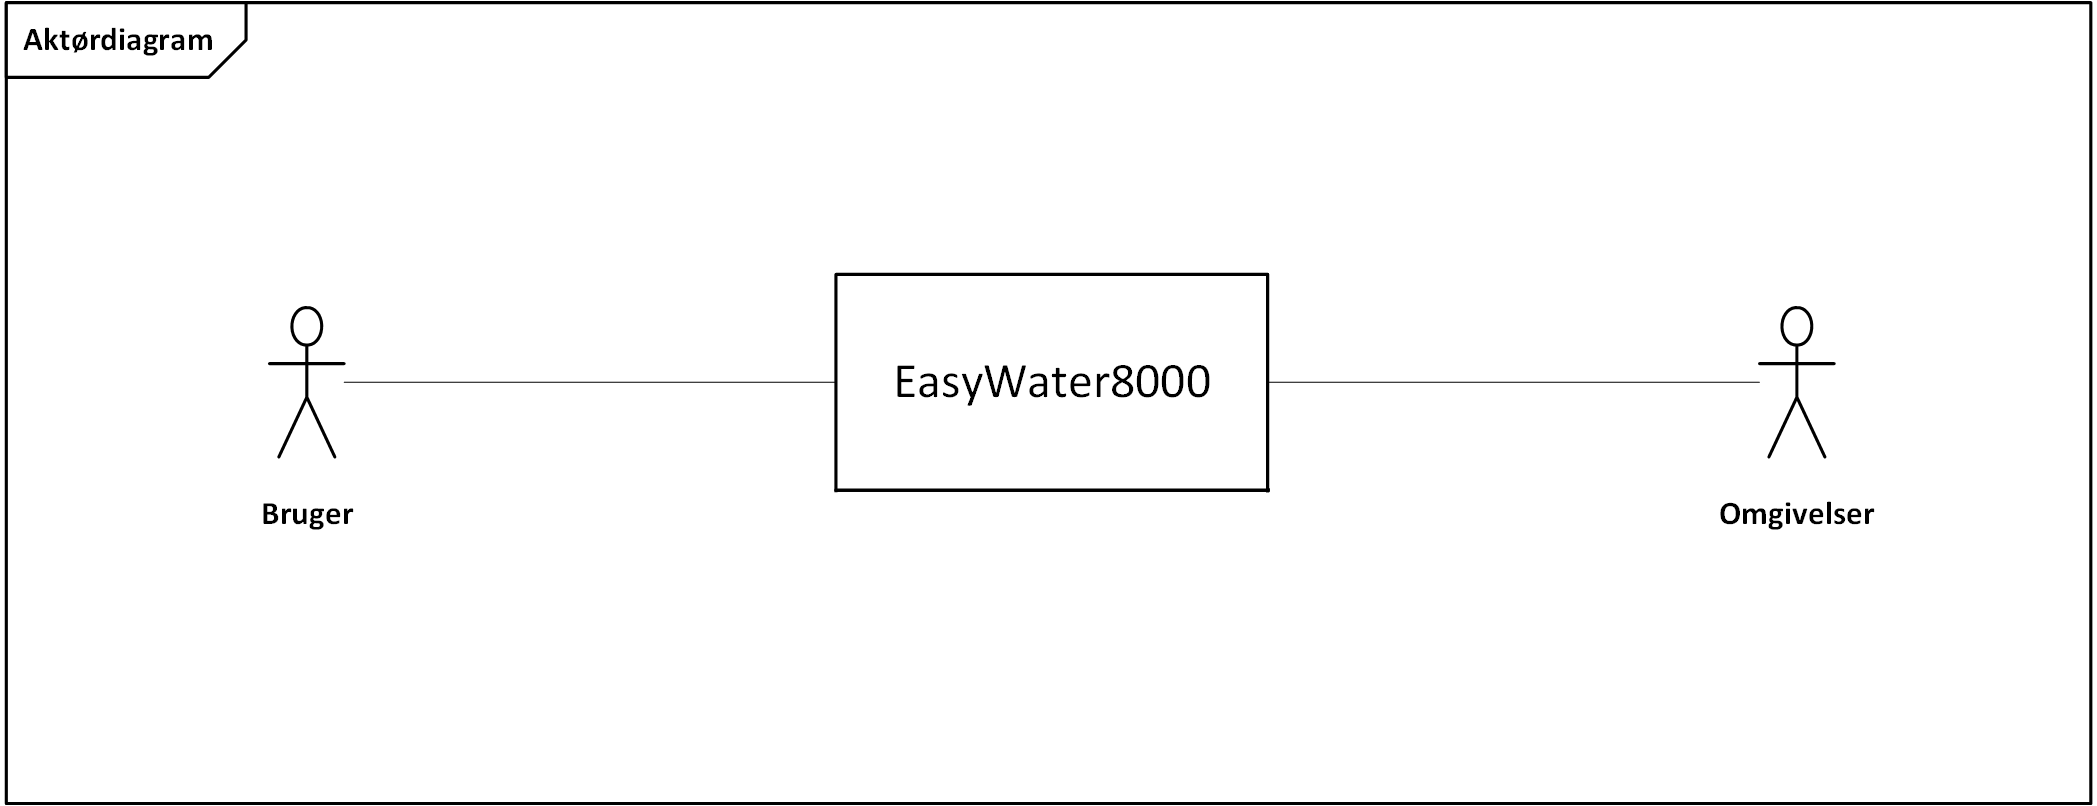
\includegraphics[width=0.9\textwidth]{filer/kravspec/visio/Kontekst_Diagram}}
\caption{Kontekst diagram}
\label{lab:kontekstdiagram}
\end{figure}

\begin{table}[!htbp] \centering
	\begin{tabular}{|p{2.5cm}|p{11.5cm}|}
	\hline
		\textbf{Aktør navn} & \textbf{Beskrivelse} \\\hline
		Bruger & Bruger vil normalt være greenkeeperen. Det er vedkommende som kontrollerer og betjener systemet. (Primær) \\\hline

		Golfbane & De almene omgivelser på golfbanen, som har indflydelse på systemets sensorer. Det indebærer temperatur, fugtighed og bevægelse i området omkring systemet. (Sekundær) \\\hline
	\end{tabular}
\end{table}

